\icode{E-MD-CA-L3-261112-006}
如图所示的装置，5个相同的木板紧挨着（不粘连）静止放在水平地面上，每块木板的质量均为 \(m =\) \,\qty{1}{kg}，长 \(l =\) \,\qty{1}{m}。它们与地面间的动摩擦因数 \(\mu_1 = 0.1\)，现有质量为 \(M =\) \,\qty{2.5}{kg}的小铅块（可视为质点），以 \(v_0 =\) \,\qty{4}{m/s}的初速度从左端滑上木板1，它与木板的动摩擦因数 \(\mu_2 = 0.2\)，取 \(g =\) \,\qty{10}{m/s}，最大静摩擦力等于滑动摩擦力。则小铅块\paren[]

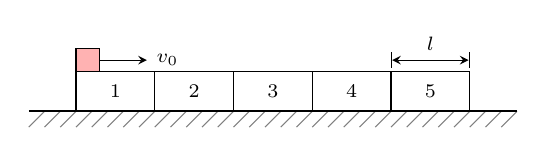
\begin{tikzpicture}[>=stealth,font=\scriptsize]
	\foreach \x in {1,...,5}{
		\draw (\x,0)--++(0,.5)--++(1,0);
		\node at({\x+.5},.25){\(\x\)};}
	\draw (6,.5)--(6,0);
	\draw[fill=red!30] (1,.5) rectangle(1.3,.8);
	\draw[->] (1.3,.65)--++(.6,0)
	node[right]{\(v_0\)};
	\draw[|<->|] (5,.65)--node[above]{\(l\)}(6,.65);
	\foreach \x in {.4,.6,...,6.6}
		\draw[gray] (\x,-.2)--++(.2,.2);
	\draw[thick] (.4,0)--(6.6,0);
\end{tikzpicture}
\begin{choices}
	\item 刚滑上木板1时，木板1会滑动 
	\item 滑离木板3之前，所有木板均处于静止状态
	\item 滑离木板3时的速度大小为1 m/s
	\item 最终停在木板5上
\end{choices}
\begin{answer}
	B

	提示：铅块在同木板上时木板与地面的最大静摩擦力是不同的。在\(1\)上时最大静摩擦力\(f_{\max 1}\)
	\[
		f_{\max 1} = \mu_1(m + M)g + \mu_1\cdot 4mg
	\]
	在\(2\)上时最大静摩擦力\(f_{\max 2}\)
	\[
		f_{\max 2} =\mu_1(m + M)g +\mu_1\cdot 3mg
	\]
	故当滑上第\(n\)块时的最大静摩擦力\(f_{\max n}\)
	\[
		f_{\max n} =\mu_1Mg + (6 - n)\cdot\mu_1mg
	\]
	当\(f_{\max n} \leq f_2 =\mu_2Mg\)时，木板滑动，\(n \geq 3.5\)。在铅块滑离\(3\)之前，木板都不动。
	\[
		v_3^2 - v_0^2 =- 2\mu_2g\cdot	
	\]
	\(v_3 =\) \,\qty{2}{m/s}。滑上\(4\)后铅块木板\(v - t\)图像如图所示，

\begin{tikzpicture}[>=stealth,font=\scriptsize]
	\draw[->,blue] (0,0)node[below left]{\(O\)}--(3,0)node[below]{\(t\)/\qty{}{s}};
	\draw[->,blue] (0,0)--(0,3)node[right]{\(v\)/(\qty{}{m\cdot s^{-1}})};
	\draw[magenta] (0,2)node[left,blue]{\(2\)}--({16/9},{2/9})coordinate(a);
	\draw[red,dashed] (0,0)--(a);
	\draw[cyan,dash dot] (a)--({20/9},0)node[below,blue]{\(\frac{10}{9}\)};
	\draw[dotted] (0,0|-a)node[left,blue]{\(\frac{2}{9}\)} --(a)--(a|-0,0)node[below,blue]{\(\frac{8}{9}\)};
\end{tikzpicture}
\end{answer}